\chapter{Implementation and Realization}

\section*{Introduction}
\addcontentsline{toc}{section}{Introduction}

This chapter presents the implementation state of Football OS at the end of the
internship period. It covers the software environment, the implemented
solution, the main graphical interfaces, and the deployment and integration
setup.

Beyond listing delivered features, the chapter analyzes how implementation
choices translated architectural intentions into executable workflows and what
technical compromises were required during integration.

\section{Development Environment}

\subsection{Software Environment}

This subsection summarizes the software stack used to implement and run
Football OS during the internship period.

\begin{table}[!htbp]
\centering
\caption{Software environment used for implementation}
\label{tab:software-environment}
\normalsize
\renewcommand{\arraystretch}{1.18}
\setlength{\tabcolsep}{5pt}
\begin{tabularx}{\textwidth}{|L{3.4cm}|C{2.1cm}|Y|}
\hline
\textbf{Technology} & \textbf{Version} & \textbf{Use in project} \\
\hline
Java & 21 & Backend language for Gateway, Governance, Workspace, and SDK modules. \\
\hline
Node.js & 20+ & Frontend runtime and build environment for Angular development. \\
\hline
Angular & Project & Frontend framework for the workspace application. \\
\hline
TypeScript & Project & Typed language for frontend development. \\
\hline
Tailwind CSS & Project & Utility-first CSS framework for interface styling. \\
\hline
Spring Boot & Project & Backend framework for the API Gateway and domain services. \\
\hline
PostgreSQL & Project & Relational database for governance data (actors, roles, players, teams, audit). \\
\hline
MongoDB & Project & Document database for workspace aggregates (documents, events, notifications, metadata). \\
\hline
Keycloak & Project & Identity and access management for authentication and user sessions. \\
\hline
Open Policy Agent & Project & Policy engine used to evaluate authorization rules. \\
\hline
Apache Kafka & Project & Messaging platform for asynchronous events and operational signals. \\
\hline
MinIO & Project & Object storage for uploaded files and edited document versions. \\
\hline
OnlyOffice & Project & Online document editor for viewing and editing workspace documents. \\
\hline
Docker / Docker Compose & Project & Local multi-service deployment and infrastructure orchestration. \\
\hline
Git / GitHub & Project & Version control and source-code collaboration. \\
\hline
Visual Studio Code / IntelliJ IDEA & Project & Development environments for frontend and backend. \\
\hline
PlantUML / Draw.io & Project & Tools used to create UML and architecture diagrams. \\
\hline
\end{tabularx}
\normalsize
\end{table}

\section{Implementation Overview}

Football OS was implemented as a distributed backend platform connected to an
Angular workspace frontend through the API Gateway. The implementation provides
an operational baseline for protected access, document workflows,
calendar/events, notifications, search, player profiles, and
OnlyOffice-based document editing. Tables~\ref{tab:software-environment}
and~\ref{tab:implementation-status} summarize the technical stack and
delivered scope.

\begin{table}[ht]
\centering
\caption{Implementation overview by feature}
\label{tab:implementation-status}
\small
\renewcommand{\arraystretch}{1.10}
\setlength{\tabcolsep}{4pt}
\begin{tabularx}{\textwidth}{|L{3.0cm}|Y|Y|C{2.2cm}|}
\hline
\textbf{Feature} & \textbf{Backend support} & \textbf{Frontend support} & \textbf{Status} \\
\hline
Authentication and secured access & Token validation and secured routing with identity propagation. & Login flow and protected routes. & Implemented \\
\hline
Document management & Document APIs, policy checks, and metadata lifecycle. & Authorized document list/detail workflows. & Implemented \\
\hline
Document versioning & Version entities and storage references. & Version access in document workflows. & Implemented \\
\hline
OnlyOffice integration & Editor configuration and save callbacks. & Embedded editor launch from document actions. & Implemented \\
\hline
Calendar/event management & Event APIs with validation and authorization. & Calendar and event-detail interfaces. & Implemented \\
\hline
Player profile consultation & Canonical/workspace aggregation with policy filtering. & Profile consultation and tab navigation. & Partial \\
\hline
Notifications & Notification generation and retrieval services. & Notification display and state updates. & Implemented \\
\hline
Search & Search endpoints with access-aware filtering. & Search entry points in workspace modules. & Implemented \\
\hline
Authorization integration & Governance policy decisions and backend checks. & UI gating by role and permission context. & Implemented \\
\hline
Storage integration & MongoDB metadata and MinIO object storage separation. & Upload/open workflows via backend-issued links. & Implemented \\
\hline
\end{tabularx}
\normalsize
\end{table}

Implementation details and technology usage remain aligned with the official
documentation references cited in this report.

The implemented baseline favors coherence over maximal feature breadth:
integration-critical capabilities (secure routing, policy checks, storage
separation, and event propagation) were stabilized first, while some advanced
functional refinements remain intentionally partial.

\subsection{Gateway and Secured Routing}

The frontend sends API requests to port 8080 (Gateway) instead of directly
calling internal services. The Gateway centralizes entry control, propagates
authenticated context, and routes workspace endpoints to Workspace Service and
actor/canonical/policy endpoints to Governance Service.

This routing strategy reduced duplication of security filters across services
and simplified frontend integration contracts. Its trade-off is stronger
dependency on Gateway configuration quality and runtime availability.

\subsection{Document Storage and Versioning}

Document metadata (category, state, ownership, version references) is stored in
MongoDB, while binary file content is stored in MinIO. Versions are represented
as separate records linked to a logical document. Online edits can create a new
version and update related metadata, preserving document history.

In a typical upload flow, Workspace verifies permissions through Gateway,
stores binary content in MinIO, persists metadata and version references in
MongoDB, and archives by state transition rather than hard deletion.

Separating metadata from binaries improved lifecycle traceability and reduced
database bloat, but it also required explicit reconciliation logic between
document records and object-storage references.

\subsection{OnlyOffice Integration}

Workspace generates the OnlyOffice editor configuration in a controlled context.
The document is opened through secure backend-managed access parameters. Save
callbacks update version metadata and content references. Access remains
enforced by backend policy decisions \cite{onlyoffice-doc}.

When a user opens or saves a document, Workspace verifies authorization before
issuing editor configuration and registers callback results as a new version.

Compared with a file download-only approach, integrated editing improves
operational continuity for staff users. The cost is additional integration
complexity, particularly around callback reliability, token scope, and version
conflict handling.

\subsection{Event Workflow Example}

A typical event workflow starts when the Head Coach creates an event from the
calendar interface. The frontend sends the request through the Gateway to the
Workspace Service. Workspace validates the event data, checks authorization,
then stores the event aggregate in MongoDB with its schedule, attendees, tasks,
and required documents. If the event affects other users, notification entries
are generated so that concerned staff members can consult the update from the
workspace.

\subsection{Technical Challenges Encountered}

The implementation phase also involved several integration challenges caused by
the distributed nature of the platform. These issues were useful for validating
the architectural choices because they required stable service communication,
consistent identity propagation, policy debugging, and coordination between
metadata and binary storage.

\begin{table}[ht]
\centering
\caption{Technical challenges encountered during implementation}
\label{tab:implementation-technical-challenges}
\small
\setlength{\tabcolsep}{4pt}
\renewcommand{\arraystretch}{1.08}
\begin{tabularx}{\textwidth}{|L{3.2cm}|L{4.3cm}|Y|}
\hline
\textbf{Challenge} & \textbf{Impact} & \textbf{Resolution} \\
\hline
Docker networking & Services needed stable local communication across containers and local processes. & Standardized local ports and routed frontend traffic through the API Gateway. \\
\hline
Keycloak role mapping & Multiple emitted roles could affect actor-context extraction and authorization behavior. & Role extraction was normalized in the backend security context. \\
\hline
OnlyOffice callback handling & Editor save operations required backend-managed versioning instead of direct file replacement. & Save callbacks were linked to document version creation and metadata updates. \\
\hline
Policy debugging & Access rules had to match role, action, resource type, and document category combinations. & Policy checks were isolated through Governance and OPA-backed decisions. \\
\hline
Multi-storage design & Metadata and binary files had to remain separated while preserving traceability. & MongoDB stores document metadata and version references, while MinIO stores binary file versions. \\
\hline
\end{tabularx}
\normalsize
\end{table}

These challenges confirmed the need for clear service boundaries and reusable
SDK abstractions, especially for security context, policy evaluation, storage
access, and event propagation.

From an engineering standpoint, the integration phase validated that the chosen
architecture was feasible for the target scope, while also revealing that
operational robustness depends on disciplined configuration management and
cross-service observability.

\clearpage
\section{Main Graphical Interfaces}

\subsection{Authentication Interface}

\begin{figure}[!htbp]
    \centering
    
\includegraphics[width=0.72\textwidth]{images/frontend/authentification.png}
    \caption{Authentication interface}
    \label{fig:authentication-interface}
\end{figure}

The interface in Figure~\ref{fig:authentication-interface} represents the
security boundary from the user perspective. Authentication gates access to
protected modules, and the resulting session context is reused for backend
authorization. The post-login redirection to the calendar supports immediate
operational orientation.

\subsection{Document Management Interface}

\begin{figure}[!htbp]
    \centering
    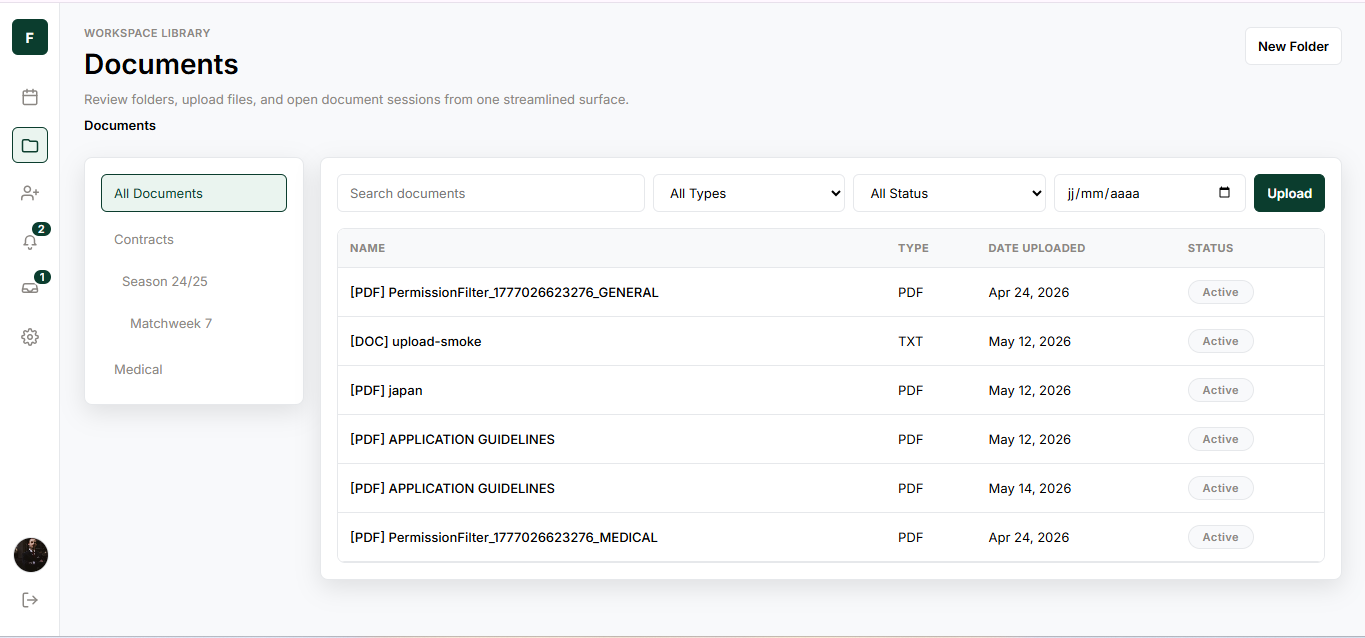
\includegraphics[width=0.72\textwidth]{images/frontend/document.png}
    \caption{Document management interface}
    \label{fig:document-management-interface}
\end{figure}
Figure~\ref{fig:document-management-interface} emphasizes the integration of
consultation, upload, organization, and archive actions in one governed
workspace. Access constraints are aligned with role and document category so
that operational convenience does not bypass policy enforcement.

\Needspace{18\baselineskip}
\subsection{Online Document Viewer and Editor}

\begin{figure}[H]
    \centering
    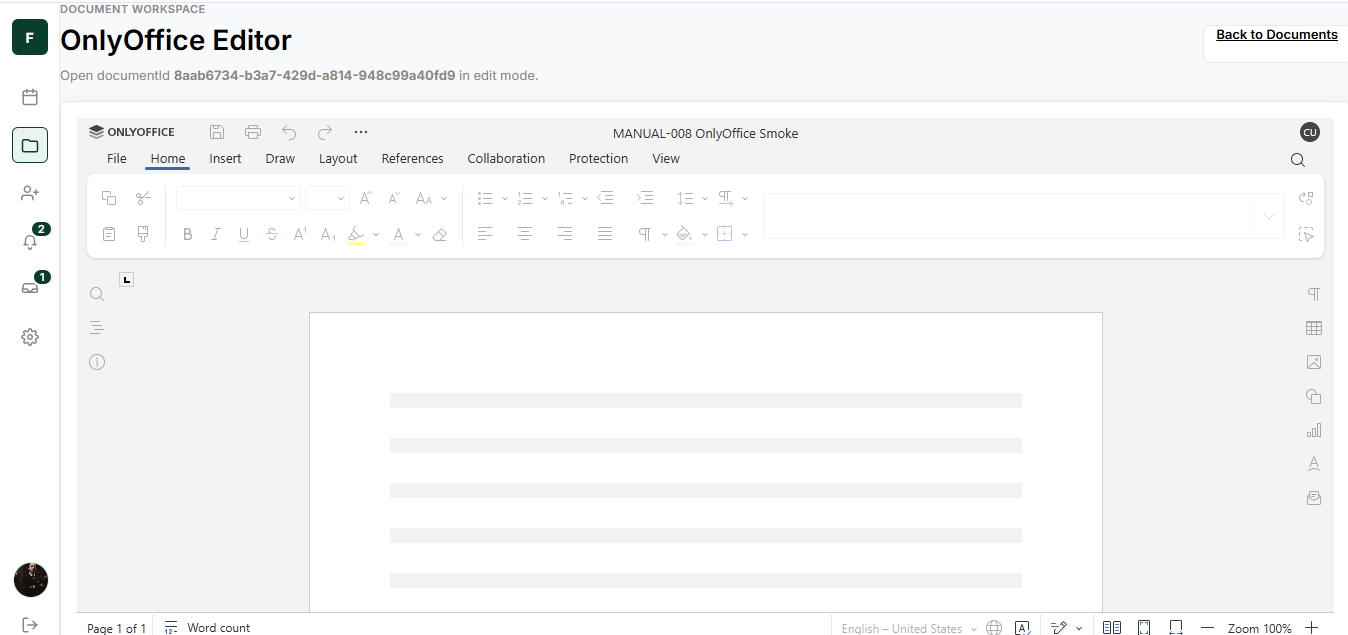
\includegraphics[width=0.72\textwidth]{images/frontend/onlyoffice-editor.png}
    \caption{OnlyOffice editor interface}
    \label{fig:onlyoffice-editor-interface}
\end{figure}

Figure~\ref{fig:onlyoffice-editor-interface} illustrates how online editing is
embedded without delegating security ownership to the editor itself. Access
decisions remain backend-driven, and document loading relies on controlled
temporary links.

\subsection{Calendar Interface}

\begin{figure}[!htbp]
    \centering
    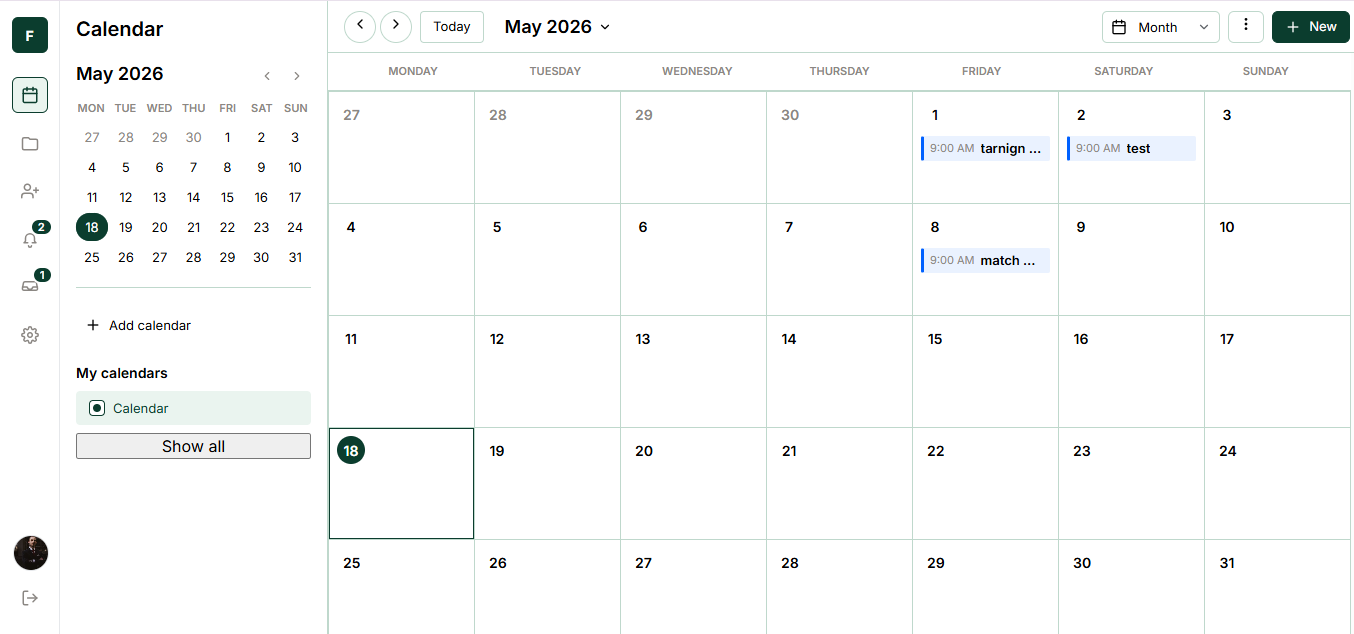
\includegraphics[width=0.58\textwidth]{images/frontend/calander.png}
    \caption{Calendar interface}
    \label{fig:calendar-interface}
\end{figure}

As presented in Figure~\ref{fig:calendar-interface}, the calendar view acts as
an operational coordination hub. Authorized users can create, update, or
archive events according to policy outcomes, while event details maintain the
link between planning data and execution artifacts (attendees, tasks, notes,
and required documents).

\subsection{Player Profile and Notifications}

Player-profile consultation remains available in the workspace and displays
role-filtered operational and document-related information, especially for
sensitive medical or administrative categories. Operational notifications are
also accessible from the workspace interface for updates such as event changes
and task assignments.

\section{Deployment and Integration}

Football OS was tested in a local Docker-based environment. The deployment
includes backend services and infrastructure containers. This setup allows
integration testing of routing, authorization, storage, messaging, and document
editing workflows.

\begin{table}[ht]
\centering
\caption{Deployment and integration components}
\label{tab:deployment-integration}
\small
\setlength{\tabcolsep}{4pt}
\renewcommand{\arraystretch}{1.10}
\begin{tabularx}{\textwidth}{|L{3.8cm}|C{1.8cm}|Y|}
\hline
\textbf{Service} & \textbf{Port} & \textbf{Role} \\
\hline
API Gateway & 8080 & Routes frontend requests to backend services. \\
\hline
Governance Service & 8081 & Manages users, roles, permissions, canonical data, and audit. \\
\hline
Workspace Service & 8082 & Manages documents, events, notifications, search, and player profiles. \\
\hline
Workspace Frontend & 4200 & Angular user interface; calls backend APIs through the Gateway. \\
\hline
PostgreSQL & 5432 & Stores governance structured data. \\
\hline
MongoDB & 27017 & Stores workspace data. \\
\hline
MinIO & 9000/9001 & Stores document files and object administration data. \\
\hline
Keycloak & Docker Compose & Provides authentication. \\
\hline
OPA & 8181 & Evaluates authorization policies. \\
\hline
Kafka & 9092 & Supports asynchronous event communication. \\
\hline
OnlyOffice & Docker Compose & Provides document viewing and editing. \\
\hline
\end{tabularx}
\normalsize
\end{table}

The deployment matrix confirms that frontend traffic remains Gateway-mediated.
This preserves consistent edge controls, but also means local troubleshooting
must consider Gateway routing and infrastructure dependencies before attributing
failures to business services alone.

\section*{Conclusion}
\addcontentsline{toc}{section}{Conclusion}

This chapter detailed the software environment, implementation overview, main
graphical interfaces, and deployment/integration of Football OS. The
implemented product provides secured access to workspace features such as
document management, calendar events, player profile consultation,
notifications, search, and online document editing.
